
%(BEGIN_QUESTION)
% Copyright 2006, Tony R. Kuphaldt, released under the Creative Commons Attribution License (v 1.0)
% This means you may do almost anything with this work of mine, so long as you give me proper credit

En elektronisk differansetrykktransmitter med fjernmonterte (kjemiske) seals brukes til å måle nivået av væske i denne trykksatte beholderen.  Spesifikk vekt (SG) for fyllevæsken i begge fjernseals er 0.934.  Måleområdet for nivået er 0 til 24 fot, og utgangssignalområdet er 4 til 20 mA.  Anta en kalibreringstoleranse på +/- 0.25 prosent.  Fullfør følgende verditabell for denne transmitteren.  Vis ligningene som brukes for å beregne alle verdier gitt prosent av spenn ($x$):

$$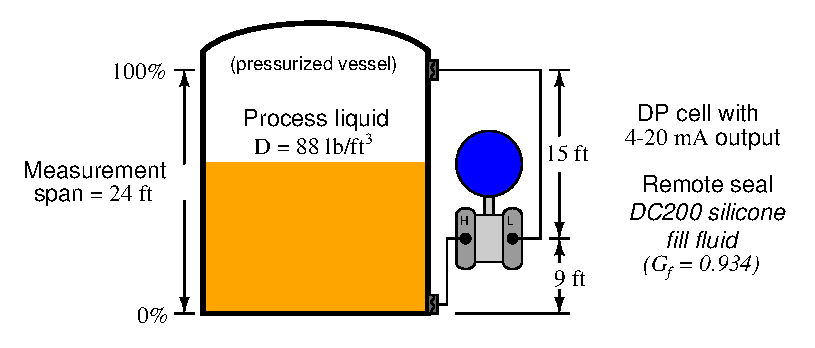
\includegraphics[width=15.5cm]{i00033x01.eps}$$

% No blank lines allowed between lines of an \halign structure!
% I use comments (%) instead, so that TeX doesn't choke.

$$\vbox{\offinterlineskip
\halign{\strut
\vrule \quad\hfil # \ \hfil & 
\vrule \quad\hfil # \ \hfil & 
\vrule \quad\hfil # \ \hfil & 
\vrule \quad\hfil # \ \hfil & 
\vrule \quad\hfil # \ \hfil & 
\vrule \quad\hfil # \ \hfil \vrule \cr
\noalign{\hrule}
%
% First row
Prosess- & Prosent av & $\Delta$-trykk & Utgangssignal & Utgangssignal & Utgangssignal \cr
%
% Another row
nivå (ft) & spenn (\%) & målt ("W.C) & ideelt (mA) & min. (mA) & maks. (mA) \cr
%
\noalign{\hrule}
%
% Another row
  & 0 &  &  &  &  \cr
%
\noalign{\hrule}
%
% Another row
  & 10 &  &  &  &  \cr
%
\noalign{\hrule}
%
% Another row
  & 25 &  &  &  &  \cr
%
\noalign{\hrule}
%
% Another row
  & 50 &  &  &  &  \cr
%
\noalign{\hrule}
%
% Another row
  & 75 &  &  &  &  \cr
%
\noalign{\hrule}
%
% Another row
  & 90 &  &  &  &  \cr
%
\noalign{\hrule}
%
% Another row
  & 100 &  &  &  &  \cr
%
\noalign{\hrule}
} % End of \halign 
}$$ % End of \vbox

\vskip 10pt

\noindent
{\bf Ligninger brukt:}

\vskip 20pt

Prosessnivå = 

\vskip 20pt

Målt trykk = 

\vskip 20pt

Utgangssignal (ideelt) = 

\vskip 20pt

Utgangssignal (min.) = 

\vskip 20pt

Utgangssignal (maks.) = 



\vfil 

\underbar{file i00033}
\eject
%(END_QUESTION)





%(BEGIN_ANSWER)

Dette er et vurdert spørsmål -- ingen svar eller hint gis!

%(END_ANSWER)





%(BEGIN_NOTES)

% No blank lines allowed between lines of an \halign structure!
% I use comments (%) instead, so that TeX doesn't choke.

$$\vbox{\offinterlineskip
\halign{\strut
\vrule \quad\hfil # \ \hfil & 
\vrule \quad\hfil # \ \hfil & 
\vrule \quad\hfil # \ \hfil & 
\vrule \quad\hfil # \ \hfil & 
\vrule \quad\hfil # \ \hfil & 
\vrule \quad\hfil # \ \hfil \vrule \cr
\noalign{\hrule}
%
% First row
Prosess- & Prosent av & $\Delta$-trykk & Utgangssignal & Utgangssignal & Utgangssignal \cr
%
% Another row
nivå (ft) & spenn (\%) & målt ("W.C.) & ideelt (mA) & min. (mA) & maks. (mA) \cr
%
\noalign{\hrule}
%
% Another row
0  & 0 & -269.0 & 4 & 3.96 & 4.04 \cr
%
\noalign{\hrule}
%
% Another row
2.4  & 10 & -228.4 & 5.6 & 5.56 & 5.64 \cr
%
\noalign{\hrule}
%
% Another row
6  & 25 & -167.5 & 8 & 7.96 & 8.04 \cr
%
\noalign{\hrule}
%
% Another row
12  & 50 & -66.01 & 12 & 11.96 & 12.04 \cr
%
\noalign{\hrule}
%
% Another row
18  & 75 & +35.49 & 16 & 15.96 & 16.04 \cr
%
\noalign{\hrule}
%
% Another row
21.6  & 90 & +96.38 & 18.4 & 18.36 & 18.44 \cr
%
\noalign{\hrule}
%
% Another row
24  & 100 & +137.0 & 20 & 19.96 & 20.04 \cr
%
\noalign{\hrule}
} % End of \halign 
}$$ % End of \vbox

\vskip 10pt

Prosessnivå = (Prosent av spenn) $\times$ 24 ft

\vskip 10pt

Målt trykk = $\left( (\hbox{Nivå} \times 12) \times {88 \over 62.4} \right) - (24 \times 12 \times 0.934)$

\vskip 10pt

Utgangssignal (ideelt) = (Prosent av spenn) $\times$ 16 mA + 4 mA 

\vskip 10pt

Utgangssignal (min.) = (Prosent av spenn) $\times$ 16 mA + 4 mA - (0.25\% $\times$ 16 mA) 

\vskip 10pt

Utgangssignal (maks.) = (Prosent av spenn) $\times$ 16 mA + 4 mA + (0.25\% $\times$ 16 mA) 

\vskip 10pt



%INDEX% Calibration: table, level transmitter
%INDEX% Measurement, level: calibration table
